\chapter{Recolección de datos de tráfico}
\label{cap:3}

Actualmente existen una variedad de tecnologías para la recolección automática de datos del tráfico. Según Mimbela y Klein \cite{mimbela2003summary} podemos dividir estas tecnologías en dos métodos. El primero, es la tecnología in-situ, que toma los datos del tráfico a través de detectores a lo largo del camino. Generalmente estas tecnologías de conteo de tráfico pueden dividirse en dos categorías: la intrusiva y la no intrusiva. Por el otro lado tenemos los datos flotantes del vehículo (FCD por sus siglas en inglés). FCD es una alternativa para obtener datos del tráfico de gran calidad y se está volviendo crucial para el desarrollo de nuevos Sistemas Inteligentes de Transporte (ITS por sus siglas en inglés).

\section{Tecnologías In-Situ}

En \cite{klein2006traffic} se puede apreciar un gran número de sensores fijos para la detección del tráfico. Estas tecnologías de detección in-situ se dividen en dos categorías: tecnologías intrusivas, que están montadas en o por debajo de la superficie de las rutas y cuya instalación ocasiona la interrupción potencial del tráfico. En contrapartida, las tecnologías no intrusivas son montadas en o por encima de la superficie de las rutas, su instalación no genera interrupción del tráfico o lo hace en pequeña medida. 

\subsection{Tecnologías Intrusivas}

Los tipos de sensores y la ubicación de los mismos se pueden observar en la \Cref{fig:intrusiva} El primer tipo de unidades son los sensores magnéticos pasivos o magnetómetros que pueden ser montados de forma permanente en hoyos a lo largo del camino, o pegados a la superficie de la ruta. Estas unidades se comunican a una estación de procesamiento cercana ya sea utilizando cables debajo del camino, o a través de comunicación inalámbrica. El sensor tiene una zona circular o elíptica de alcance de detección. Los magnetómetros monitorean la fluctuación en la fuerza del campo magnético, el cual cambia en presencia de objetos de metal moviéndose (automóviles).

\begin{figure}[h]
	\centering
	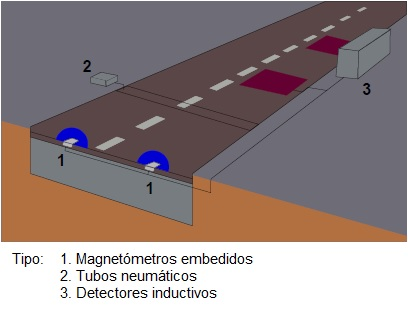
\includegraphics[width=0.7\textwidth]{capitulos/3/figuras/figura1.jpg}
	\caption{\label{fig:intrusiva} Típicas configuraciones de detección intrusiva}	
\end{figure}

El segundo tipo de de unidades utilizan tubos neumáticos que son extendidos a través de la calzada y se fijan en el lado de la acera en ambos extremos. Estos sistemas solamente se pueden implementar de forma temporal, debido a la naturaleza frágil de los tubos, que son fácilmente dañados por vehículos pesados o que se mueven a gran velocidad. Estos sensores envían una ráfaga de presión de aire a lo largo de un tubo de goma cuando un vehículo pasa por encima de los tubos. El pulso de presión de aire cierra un interruptor de aire, produciendo una señal eléctrica que es transmitida a un contador. Tienen la ventaja de ser sistemas portables utilizando plomo-ácido, gel, u otras baterías recargables como fuente de energía.

El tercer tipo son los detectores de bucle inductivos (IDL por sus siglas en inglés). Consisten en rollos de alambre recubierto, enterrados en ranuras cortadas en la superficie de la carretera y sellados con masilla bituminosa. Los datos son enviados a través de un cable enterrado con los bucles hasta una unidad de procesamiento al borde de la carretera. La zona de detección para los sensores de bucle inductivo depende de la forma de corte de la ranuras del bucle. Los IDL son una tecnología barata y madura. La oscilación de la señal eléctrica es aplicada al bucle, el metal contenido en el chasís de un vehículo en movimiento cambia las propiedades eléctricas del circuito. Estos cambios son detectados por una unidad al costado del camino, que disparan un evento de vehículo.

El cuarto tipo de sistemas intrusivos es Weigh-In-Motion (WIM) mostrado en \Cref{fig:Weight-In-Motion}, los detectores consisten en un sensor piezoeléctrico ubicado en un canal a través del camino. El sistema registra la tensión medida por los sensores y calcula la carga dinámica, la carga estática se calcula utilizando la carga dinámica y parámetros de calibración. Los parámetros de calibración dependen de factores como la velocidad del vehículo y el pavimento o la dinámica de suspensión que influencia en los cálculos de la carga estática. La precisión de los sistemas WIM puede ser expresada como función a la velocidad con que el vehículo pasa sobre las placas, asumiendo que el sistema está instalado en una carretera sujeta a las condiciones normales de tráfico Estos sistemas son raros y se utilizan en ubicaciones específicas mayormente para el control de acceso.

\begin{figure}[h]
	\centering
	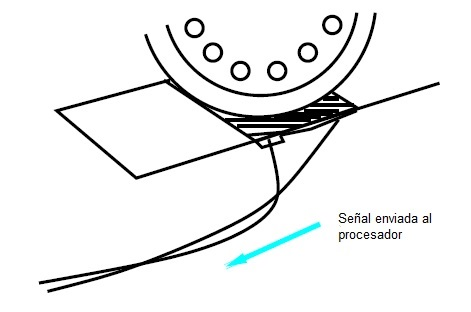
\includegraphics[width=0.7\textwidth]{capitulos/3/figuras/figura2.jpg}
	\caption{\label{fig:Weight-In-Motion}  Sistema de detección Weight-In-Motion}	
\end{figure}

\subsection{Tecnologías No Intrusivas.}

Las tecnologías no intrusivas incluyen recolección de datos por video, detectores infrarrojos pasivos o activos, radares de microondas, detectores ultrasónicos, detectores acústicos, detectores láser y fotografía aérea. Según el Dr. Mathew \cite{mathew2014transportation}, todas estas tecnologías representan campos emergentes que se están expandiendo rápidamente con continuos avances en el procesamiento de señales. Actualmente estas tecnologías son utilizadas para proveer información suplementaria para lugares seleccionados o para aplicaciones específicas. La Mayoría de los sistemas no intrusivos son operacionalmente y en cierta medida visualmente similares, consistiendo en pequeñas unidades electrónicas montadas en contenedores a prueba de agua y colocadas en varias ubicaciones con se puede observar en la \Cref{fig:noIntrusica}.

\begin{figure}[h]
	\centering
	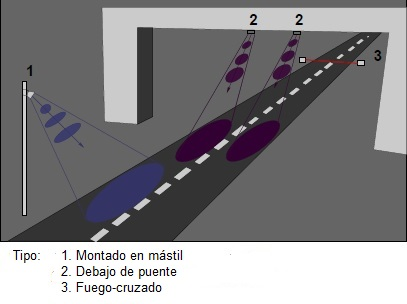
\includegraphics[width=0.7\textwidth]{capitulos/3/figuras/figura3.jpg}
	\caption{\label{fig:noIntrusica}  Configuraciones típicas de tecnologías no intrusivas}	
\end{figure}

El primer tipo de detectores no intrusivos son los montados al costado de la carretera. El detector procesa un campo de visión que cubre un área oblicua ya sea por encima o por debajo de la unidad. También existen múltiples zonas de detección definidas dentro del campo de visión,  o la zona total de detección al igual que el campo de visión, dependiendo del tipo de detector específico y la tecnología utilizada.

Problemas de oscurecimiento ocurren cuando vehículos grandes cubren a vehículos pequeños del detector o cuando el campo de visión es muy grande, llevando a detección de vehículos afuera del carril deseado. El segundo tipo de detectores no intrusivos son montados debajo de puentes o portales, con un campo de visión justo por debajo de los mismos, o ligeramente oblicuo a la unidad. Finalmente, algunas unidades como los monitores de polución de camino abierto son montados a nivel del piso a los lados del camino, disparando un haz a través de la carretera. Estas unidades están sujetas al enmascaramiento de lado a lado y por lo tanto, son más adecuadas para un solo carril.

En la detección por imagen de video los parámetros del tráfico son recolectados a través del análisis cuadro por cuadro de las imágenes capturadas por las cámaras al costado del camino. Dependiendo de la tecnología de procesamiento, se pueden obtener prácticamente todos los parámetros del tráfico a través de análisis de video. Un problema con este sistema es que es susceptible al oscurecimiento y su rendimiento puede decaer con el mal clima o con bajas condiciones de luz.

Los sensores infrarrojos pueden montados por encima o al costado del tráfico dependiendo de la información que se quiera obtener con ellos. Estos sensores son utilizados para obtener el volumen, la velocidad y el tipo de vehículos, como también a los transeúntes. Tienen la ventaja de ser menos susceptibles al mal clima. Cuando los sensores poseen una baja resolución la precisión en la velocidad y el largor de los vehículos tiende a ser bastante impreciso.

\section{Tecnologías en vehículo o Floating Car Data (FCD)}

En adición a la utilización de tecnologías in-situ, muchas aplicaciones de gestión de redes de tráfico utilizan dispositivos en los vehículos, generalmente conocidos como sistemas de ubicación automática de vehículo (AVL por sus siglas en inglés). Los dispositivos AVL proveen información de posición cuando un vehículo equipado con ellos pasa cierto punto de la red, o información continua a medida que el vehículo viaja a través de la red. Los anteriores sistemas se basaban en vehículos equipados con transpondedores que transmitían y recibían información de los dispositivos ubicados en la carretera. Los sistemas actuales se basan en la tecnología del Sistema de Posicionamiento Global (GPS por sus siglas en inglés).

El principio de FCD es recolectar datos de tráfico en tiempo real ubicando los vehículos a través de teléfonos móviles o GPS en toda la red de caminos como se muestra en la \Cref{fig:ComunicacionGPS}. Todos los vehículos equipados con con teléfonos móviles o con GPS actuarán como sensores para la red de caminos. Datos como la ubicación del vehículo, la velocidad y dirección del viaje son enviados de forma anónima un un centro de procesamiento. Después de la recolección y extracción, información útil como el estado del tráfico y rutas alternativas pueden ser distribuidas a los conductores del camino. FCD es una alternativa o más bien una fuente de información de alta calidad para las tecnologías existentes. Ayuda a mejorar la seguridad, eficiencia y confiabilidad de los sistemas de transporte. Se están volviendo cruciales en los Sistemas Inteligentes de Transporte (ITS por sus siglas en inglés).

\begin{figure}[h]
	\centering
	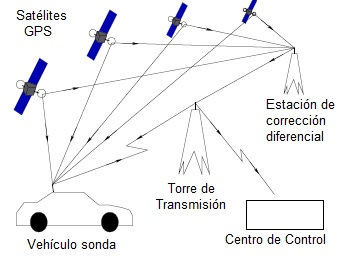
\includegraphics[width=0.7\textwidth]{capitulos/3/figuras/figura4.jpg}
	\caption{\label{fig:ComunicacionGPS}  Comunicación con GPS}	
\end{figure}

\subsection{FCD basado en GPS}

La tecnología GPS se está convirtiendo cada vez más útil y barata, va en aumento el número de autos equipados con sistemas GPS que le permiten ser ubicados dentro de la red de caminos. La precisión de la ubicación del vehículo es relativamente alta, típicamente menor a 30 metros. Generalmente, los datos del tráfico se obtienen de vehículos privados o camiones son más adecuados para autopistas y zonas rurales.

Actualmente, los datos de sondas GPS son utilizados como fuente para información en tiempo real de muchos proveedores de servicios pero sufre el limitado número de vehículos equipados y los costos de equipamiento comparados con el FCD obtenido de teléfonos celulares.

\subsection{Identificación por radiofrecuencia o sistemas de transpondedores}

La identificación por radiofrecuencia (RFID por sus siglas en inglés)  es un método automático de identificación, confiando en el almacenamiento y recuperación de datos de áreas remotas utilizando dispositivos llamados etiquetas RFID o transpondedores. La tecnología requiere la cooperación entre lectores y etiquetas RFID. Una etiqueta RFID es un objeto que puede ser aplicado o incorporado a un producto, animal, o persona para el propósito de identificación y seguimiento utilizando ondas de radio. Algunas etiquetas pueden ser leídas desde varios metros de distancia y más allá de la línea de vista del lector.

Una etiqueta RFID se compone de un microchip para recolectar información y de una antena que transmite estos datos de forma inalámbrica a un lector. En su forma más básica, el chip contendrá un identificador serializado, o el número de matrícula, que identifica de manera única al objeto.

\subsection{FCD basado en teléfono móviles}

La rápida expansión de los teléfonos inteligentes y los múltiples sensores que poseen los mismos, los convierte en una fuente invaluable para la obtención de FCD. En los últimos tiempos un gran número de trabajos se centró en la utilización de dispositivos móviles para la detección del tráfico. La mayoría de los mismos aprovechando los sistemas de GPS, pero también han habido otros que utilizan las redes GSM, WiFi y hasta la tecnología bluetooth.

Ya en 2007, Scott Fraser \cite{fraser2007use} habla de la viabilidad de utilización de dispositivos móviles como alternativa a los métodos típicos de detección de tráfico. En aquel entonces uno de los problemas grandes encontrados era la precisión, ya que se utilizaba la triangulación de antenas (\Cref{fig:triangulacionAntenas}) como método de ubicación, y el mismo tiene una precisión entre 50 y 200 metros. Posteriormente, con la llegada de los sistemas GPS a los teléfonos inteligentes se mejoró bastante el problema de la precisión.

\begin{figure}[h]
	\centering
	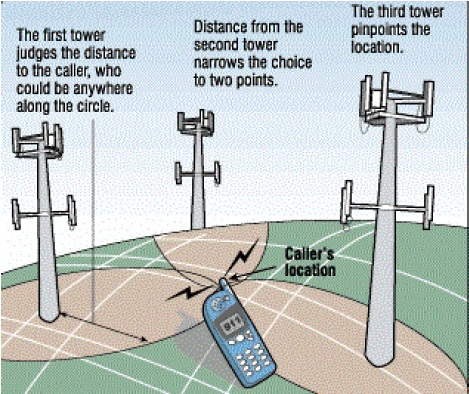
\includegraphics[width=0.7\textwidth]{capitulos/3/figuras/figura5.jpg}
	\caption{\label{fig:triangulacionAntenas} Triangulación de Antenas}	
\end{figure}

A pesar de la baja precisión de los sistemas GSM para la ubicación de dispositivos móviles, se han realizado trabajos como CTrack \cite{thiagarajan2011accurate} que utiliza solamente este método de triangulación de antenas celulares en lugar de GPS o WiFi que bien es sabido consumen un alto nivel de batería. En este método el consumo marginal de energía es cercano a cero. CTrack utiliza un nuevo Modelo Oculto de Markov de dos pasos que secuencia las huellas digitales GSM de los celulares sin convertirlas en coordenadas geográficas, y los fusiona con los datos de los sensores de bajo consumo de energía con los que cuentan la mayoría de los teléfonos inteligentes, incluyendo acelerómetros (para detectar movimiento) y compases magnéticos (para detectar giros). El sistema consiste en dos componentes de software, la librería para el teléfono y el servicio web. La librería recolecta, filtra y escanea los datos obtenidos de GSM y de otros sensores del teléfono y los transmite a través de cualquier red inalámbrica disponible al servicio web, que corre un algoritmo de mapeo de trayectoria sobre los datos recibidos.

Otro trabajo que busca un uso eficiente de energía es EnAcq \cite{fang2011enacq}. El mismo presenta un nuevo método de adquisición de ubicaciones basado en un pareo de mapas mejorado que se centra en dos desafíos claves: datos imprecisos de trayectoria y consumo de energía. Para mejorar la precisión de los datos de la trayectoria, utiliza un algoritmo mejorado de pareo de mapas basado en modelos ocultos de Markov, que puede encontrar pares candidatos para cada punto sin usar una consulta de rango y determinar la ruta más probablemente seguida por el vehículo. Para evitar el consumo innecesario de energía, utiliza un periodo adaptativo para la toma de ubicaciones por GPS, este periodo de toma de posiciones se basa en el estado de movimiento actual del vehículo.

También existen trabajos que utilizan otros métodos para detectar la ubicación de los vehículos como la la tecnología Bluetooth y las redes WiFi \cite{ruppe2012augmenting}. Donde se ven enfoques de bajo coste y gran escala para monitorear el tráfico, que aumentan el principio de FCD y permiten la detección de vehículos, transeúntes, ciclistas y pasajeros del transporte público para lograr datos espacio-temporales de tráfico por un aumento considerable de la base de datos subyacente. 

Este nuevo enfoque se basa en un método para la ubicación anónima a través de la detección indirecta de objetos de tráfico (autos, ciclistas. transeúntes) usando las tecnologías WiFi y Bluetooth. Esto es ventajoso debido a que varios participantes del tráfico utilizan dispositivos con el WiFi o Bluetooth activado. Por ejemplo, un auto que está equipado con receptores específicos, detecta todos los objetos de tráfico que están dentro de un área a través del número de identificación de WiFi o Bluetooth. Este número de identificación se ve aumentado por las marcas de tiempo y la ubicación de los objetos de detección. Los datos medidos son procesados para obtener las trayectorias, tiempo de viaje, estado del tráfico, matrices de origen-destino y otros parámetros de tráfico.

\section{Sistemas Inteligentes de Transporte (ITS)}

Los Sistemas Inteligentes de Transporte son la aplicación de tecnologías de computación, electrónica y comunicaciones con estrategias de administración de una forma integrada para proveer información de viaje para incrementar la seguridad y eficiencia de los sistemas de transporte en las rutas. Estos sistemas incluyen vehículos, conductores, pasajeros, operadores de rutas y administradores, todos interactuando los unos con los otros y enlazándose con la compleja infraestructura de los sistemas para mejorar la seguridad y capacidad de las rutas. Chowdhary y Sadek \cite{chowdhury2003fundamentals} hablan de los servicios al usuario, la arquitectura y el planeamiento de los ITS, que utilizados correctamente mejoran la seguridad y movilidad en el transporte y realzan la conectividad global en términos de mejoras en la productividad logradas a través de la integración de avanzadas tecnologías de comunicación en la infraestructura del transporte.

\subsection{Servicios a usuarios ITS}

Con el fin de implementar ITS, se desarrolla un marco destacando los varios servicios que los ITS pueden proveer a los usuarios. Una lista de 33 servicios a los usuarios ha sido proveída en el plan nacional ITS de los Estados Unidos. El número de servicios de usuario sigue variando con el tiempo cuando un nuevo servicio es añadido. Todos estos servicios están divididos en ocho grupos. La división de estos servicios está basada en la perspectiva de la organización y la distribución de funciones técnicas comunes. Estos ocho grupos de servicios se dividen de la siguiente manera:

\begin{itemize}
\item Gestión de los viajes y el tráfico

\item Operaciones de transporte público

\item Pago electrónico

\item Operaciones de vehículos comerciales

\item Sistemas avanzados de control y seguridad de vehículos

\item Gestión de emergencias

\item Gestión de la información

\item Gestión del mantenimiento y construcción.
\end{itemize}

\subsection{Arquitectura ITS}

La arquitectura de los ITS provee un marco común para planeamiento, definición, e integración de los sistemas inteligentes de transporte. Especifica cómo los diferentes componentes de un ITS deben interactuar entre ellos para ayudar a resolver los problemas del transporte. Proporciona a los profesionales del transporte una gran variedad de opciones para hacer frente a sus necesidades. Identifica y describe varias funciones y asigna responsabilidades a las partes interesadas del ITS. La arquitectura debe cumplir con los siguientes requisitos:

Interoperabilidad, la arquitectura debe ser de tal manera que la información recolectada, la función implementada o cualquier equipo instalado pueda ser interoperable por varias agencias de diferentes regiones.

Capaza de compartir e intercambiar información. La información de las operaciones de tráfico puede ser útil en los servicios de emergencia.

Compartir recursos. torres regionales de comunicación construidas por diversas agencias privadas están obligadas a ser compartidas por las operaciones ITS.

\subsection{Planeamiento ITS}

El planeamiento ITS consiste en integrar ITS en el proceso de planeamiento del transporte. El planeamiento del transporte ayuda a dar forma a un sistema de transporte bien balanceado que pueda cumplir con las demandas futuras. Es un proceso interactivo que incluye identificación de problemas, generación de soluciones, análisis, evaluación e implementación. Esto puede ser integrado con ITS utilizando computadores, sistemas de comunicación y software. Como el planeamiento es realizado normalmente para un periodo largo, la instalación de ITS debe ser actualizable y se debe asegurar que los equipos y tecnologías serán compatibles para futuras mejoras y expansiones.

Los pasos tradicionales en un planeamiento de transporte son los siguientes:

\begin{enumerate}
\item Establecer metas y objetivos

\item Inventario de las condiciones existentes.

\item Análisis de las condiciones existentes.

\item Elementos de largo y corto alcance.

\item Pronóstico del uso de la tierra, población y empleo.

\item Pronóstico de viajes futuros.

\item Desarrollo y evaluación de planes alternativos de transporte.

\item Preparación de planes y programas recomendados.
\end{enumerate}

El proceso de planeamiento de transporte ITS difiere del tradicional, ya que los ITS tienen la capacidad única de integrar diferentes modos de transporte como el transporte público, tráfico, y elementos infraestructurales a través de comunicaciones y control. El potencial de integración multimodal ofrece una gran oportunidad para la planificación a través de los diferentes modos.
